\chapter{基于深度学习的ECDSA签名智能卡的侧信道分析方法}\label{chap:search2}{
	\section{智能卡ECDSA算法实现攻击点选择}
	
	作为研究目标的智能卡所属的产品家族(Product Family)为J3D081,它是符合ISO7816\citep{ISO/IEC7816}与ISO14443 A\citep{ISO/IEC14443}规范的双界面的JAVA产品,其JCOP版本是Java Card3.0.1,GlobalPlatform版本是2.2.1。该智能卡使用了SmartMX\citep{p5x}安全微控制器芯片。Roche等\citep{Roche21}对同样使用SmartMX的两款智能卡进行过研究,并对其在ECDSA算法中的数乘实现进行了分析和猜想。因为芯片型号完全相同,我们认为J3D081智能卡与Roche等\citep{Roche21}研究的智能卡中ECDSA中的数乘实现也相同。
	
	ECDSA签名过程使用的一次性随机数$\nonce$是敏感信息。如果它出现泄漏,那么攻击者有可能使用数学方法恢复私钥$\sk$。随机数$\nonce$泄漏越多,攻击恢复私钥的可能性越大。
	
	对于本文研究的ECDSA签名智能卡,不能直接使用侧信道攻击恢复随机数$\nonce$的泄漏。如\algorithmref{alg:improvesignscalar}所示,算法的敏感信息是$\tilde{\nonce}_i,i=0,1,\cdots, 128$,但它不存在泄漏(或泄漏程度小到不能直接利用)。我们注意到$\leakedmultiplier_i$敏感信息有关(\algorithmref{alg:improvesignscalar}第5行)且它存在可以利用的泄漏,因此可以将攻击点选为$\leakedmultiplier_i$,恢复$\leakedmultiplier_i$后可以恢复$\tilde \nonce_i$的一部分信息。
	
	\begin{figure}[!h]
		\begin{center}
			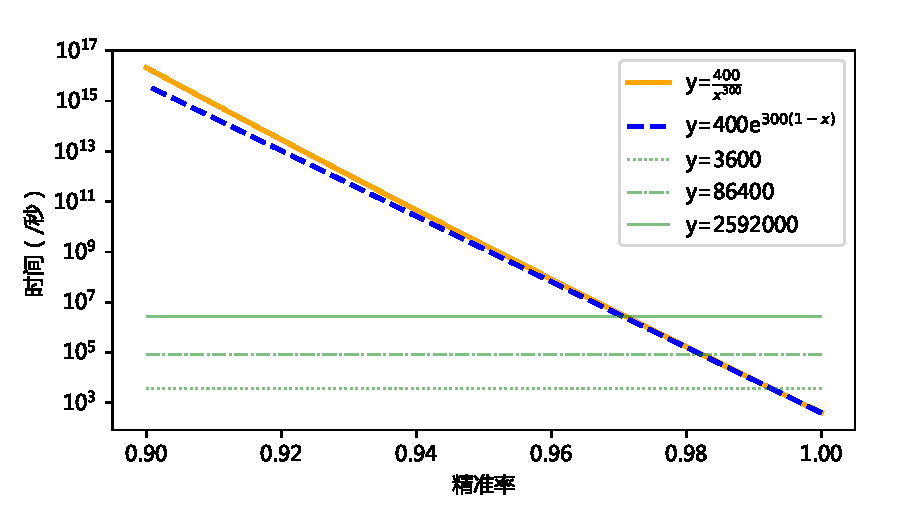
\includegraphics[width=\textwidth]{expotime}
			\bicaption{\enspace 侧信道攻击泄漏恢复准确率对攻击时间期望的影响}{\enspace Impact of SCA Leakage Recovery Accuracy on the Expectation of Attack Time}
			\label{fig:expotime}
		\end{center}
	\end{figure}
	
	需要注意的是,本研究所使用的求解算法$S$要求\textbf{用于构造方程的签名中的随机数泄漏}的准确率是100\%,而没有要求\textbf{签名中的随机数泄漏}准确率是100\%。因此,在侧信道攻击恢复泄漏的准确率略小于100\%的情况下,可以多次尝试仅使用部分泄漏并使用$S$求解。如果选取到的部分泄漏恰好没有错误,那么求解算法能求解出实际私钥$\sk$。这样带来的代价是需要消耗更多时间才能恢复实际私钥。具体来讲,在侧信道攻击恢复泄漏的准确率略小于100\%的情况下,使用多次尝试$S$的方法所消耗的时间会随着准确率的减小而成指数级增长,推导过程如\propositionref{prop:expotime}所示。\figureref{fig:expotime}展示了侧信道攻击恢复泄漏的准确率略小于100\%的情况下多次尝试$S$的方法在理论上的技术效果,其中橙色实线表示恢复实际私钥的时间的期望,蓝色虚线表示使用指数函数可以对时间期望的下限做一个很好的估计,不同线型的绿色虚线表示攻击所能容忍的不同程度时间消耗(一小时、一天、一个月)。进一步分析可以知道,如果要求使用数学方法分别在一个月、一天、一小时内恢复实际私钥,那么通过侧信道攻击所恢复的签名中的随机数泄漏的准确率分别需要达到97.12\%、98.22\%、99.27\%。

	本研究的攻击点是ECDSA签名操作中数乘实现(\algorithmref{alg:improvesignscalar})中$\leakedmultiplier_i$的泄漏,侧信道攻击最终目标是恢复足够多可利用\footnote{足够多、可利用的具体标准取决于求解算法$\mathcal S$。对于本文使用的求解算法$S$,足够多指使用75条有可利用泄漏的签名构造方程,可利用指签名中的随机数泄漏连续4比特。}的签名中的一次性随机数$\nonce$的泄漏的情况下,提高恢复的泄漏准确率。侧信道攻击恢复随机数泄漏的准确率越高,求解实际私钥所需要调用$S$的次数就越少,攻击时间也就越少。侧信道攻击恢复随机数泄漏越多,求解出实际私钥的可能性就越大。
	
	\section{智能卡ECDSA算法实现侧信道分析难点}
	本研究采集数据的参数如\tableref{tab:acquisitionpara}所示。
	
	\begin{table}[!h]
		\bicaption{\enspace J3D081采集参数}{\enspace Acquisition parameters on J3D081}
		\label{tab:acquisitionpara}
		\centering
		%\footnotesize% fontsize
		%\setlength{\tabcolsep}{4pt}% column separation
		%\renewcommand{\arraystretch}{1.2}%row space 
		\begin{tabular}{ll}
			\hline
			操作 & ECDSA签名\\
			输入 & 固定消息$m$,(随机选择的)固定私钥$d$\\
			操作次数(能量迹条数) & 5000\\
			一次数乘时间 & 约50ms\\
			采样率 & 5GHz\\
			每条能量迹采样时间 & 10ms\\
			每条能量迹采样点个数 & 50M\\
			通道 & 电磁\\
			数据大小 & 约1TB\\
			采集时间 & 约1天\\
			\hline
		\end{tabular}
	\end{table}
	
	侧信道攻击智能卡ECDSA直到恢复实际私钥分为如下多个步骤。其中,步骤一可以通过改进采集环境或采集设备提升采集到的泄漏数量,步骤二通过改进侧信道攻击方法或降低置信度提升恢复的信息泄漏数量,步骤三需要通过更强的数学工具才可能在现有基础(见\apptableref{apptab:infoonsymbol})上进一步提升恢复敏感信息泄漏的比例,步骤四无法改进,步骤五可以通过使用更好的求解算法加以改进以减少攻击时间。
	
	\begin{enumerate}
		\item [\textbf{步骤一}]采集多条签名以及对应的电磁迹;
		\item [\textbf{步骤二}]从电磁迹中恢复$\leakedmultiplier_i$的信息泄漏;
		\item [\textbf{步骤三}]从$\leakedmultiplier_i$的信息泄漏中恢复$\tilde \nonce_i$的敏感信息泄漏;
		\item [\textbf{步骤四}]从签名中过滤出所有有连续4比特泄漏的签名;
		\item [\textbf{步骤五}]每次随机选择75条签名,利用签名以及其泄漏调用$S$求解直至求解成功。
	\end{enumerate}
	
	对于步骤一,在现有实验条件下(见\tableref{tab:acquisitionpara})每条签名中数乘实现时长约50ms的电磁迹只能采集10ms,128次迭代只能采集到约30次。对于步骤二,使用自适应数据增强方法提升恢复的信息泄漏数量。步骤三、四、五不在本研究范围内,提升效果的具体方法不予赘述。
	
	本研究不考虑进一步改进步骤一、三、四、五,这使得使用侧信道分析实现步骤二需要考虑如下难点:
	
	\begin{itemize}
		\item 信息泄漏难以定位;
		\item 恢复信息泄漏真阳性率要求高\footnote{具体数值由电磁迹条数、电磁迹包含的迭代次数、从信息泄漏中恢复敏感信息泄漏的比例、求解算法$\mathcal S$对可利用敏感信息泄漏的定义、求解算法$\mathcal S$对敏感信息泄漏总量的需求、求解算法$\mathcal S$的运行时间、求解算法$\mathcal S$本身的成功率、可以容忍的攻击的时间消耗等多种因素共同决定};
	\end{itemize}

	本研究提出了一种基于时间模版的两阶段对齐解决信息泄漏难以定位的问题;本文应用了前一章的自适应数据增强方法提升恢复信息泄漏真阳性率。
	
	侧信道攻击需要恢复敏感信息泄漏的准确率高,但是对于以准确率作为评价恢复$\leakedmultiplier_i$信息泄漏效果的指标不合理。从\apptableref{apptab:infoonsymbol}可以看出攻击者只能从$\leakedmultiplier_i$的取值中分析出一次性随机数$\nonce$的某个比特$\nonce_i=0$,而无法分析出$\nonce$的任何一个比特$\nonce_i=1$。因此评价恢复$\leakedmultiplier_i$信息泄漏效果时,只用考虑在$\leakedmultiplier_i=1$时尽可能将$\leakedmultiplier_i$预测为1、在$\leakedmultiplier_i=2$时尽可能将$\leakedmultiplier_i$预测为2,而不用考虑在$\leakedmultiplier_i=3$时尽可能将$\leakedmultiplier_i$预测为3。又由于本研究使用的求解算法$S$不考虑低位的泄漏,因此本研究只考虑在$\leakedmultiplier_i=1$时尽可能将$\leakedmultiplier_i$预测为1。本研究将$\leakedmultiplier_i=1$对应的能量迹称为阳性样本,并将真阳性率作为评价恢复$\leakedmultiplier_i$信息泄漏效果的指标。
	
%	侧信道分析的第一个难点在于,敏感信息是$\tilde{k}_i$没有直接泄漏,这使得从理论上讲不可能从电磁迹泄漏中恢复所有敏感信息。从一条签恢复的回复的敏感信息越少,就需要使用越多签名构造方程才可能求解出私钥。
%	
%	
%	即使以100\%的成功率恢复所有泄漏的$t_i$,也会因无法分辨泄漏来自于算法的哪个分支(\algorithmref{alg:improvesignscalar}第5、8行),从而在理论上不能完全恢复$\tilde k_i$的信息,进而不能恢复随机数$k$的所有泄漏\footnote{因为$\left\{\tilde{k}_0,\tilde{k}_1,\dots,\tilde{k}_i,\dots, \tilde{k}_{l-1}\right\}$是$k$的编码形式,所以恢复某些$\tilde k_i$的比特等价于恢复随机数$k$的等量比特。因为$(k_0k_1k_3\dots k_{257})_2$是$k$的二进制表示,所以恢复某些$k_i$也等价于恢复随机数$k$的等量比特。}。\tableref{tab:infoonsymbol}总结了从$t_i$中所恢复的$\tilde k_i$和$k$的信息。从\tableref{tab:infoonsymbol}中可以归纳出这样的结论:
%	
%	\begin{itemize}
%		\item 如果攻击者知道$t_i=1$(有$\frac38$的概率发生),那么攻击者可以推断$\tilde k_i$的高比特是0,即$k_i=0$(见\algorithmref{alg:encodek}),无法推断$\tilde k_i$的低比特。
%		\item 如果攻击者知道$t_i=2$(有$\frac5{16}$的概率发生),那么攻击者可以推断$\tilde k_i$的低比特是0,即$k_{i+129}=0$,无法推断$\tilde k_i$的高比特。
%		\item 如果攻击者知道$t_i=3$(有$\frac5{16}$的概率发生),那么攻击者无法推断$\tilde k_i$的任意比特。
%	\end{itemize}
%	
%	
%	侧信道攻击所能恢复的是$t_i$的数值,构造方程的签名中的随机数泄漏是$\tilde k_i$的数值,这两个不能完全对应。依据前两条结论从$t_i$中推断出的随机数$k$的某些比特的值就是攻击者可以完全确定的所有随机数$k$的泄漏。这些泄漏随机地分布在随机数$k$所有位置。因此攻击者
%		
%	从\tableref{tab:infoonsymbol}中归纳的信息可以看出,对于任意一条签名中随机数$k$的任意一个比特$k_i$,不可能使用侧信道攻击得出这样的结论:有超过100\%的把握认为$k_i=1$。
%	
%	实际上,在采集的电磁迹受限的情况下,侧信道攻击恢复随机数泄漏多和侧信道攻击恢复随机数泄漏的准确率高两个目标是互相冲突的。原因在于,在采集的电磁迹受限下,可以很容易地通过提高置信度实现提高侧信道攻击恢复随机数泄漏的准确,但是这样一来会减少侧信道攻击恢复随机数泄漏。
	
	
	\section{智能卡ECDSA算法实现信息泄漏预处理方法研究}
	
	信息泄漏指的是$t_i$的泄漏。一条签名的电磁迹采样点个数达到$5\cdot10^{7}$,现有的对齐方法无法同时满足高效和准确的需求。电磁迹中每处信息泄漏的POIs少(约50个采样点),使用基于与单处信息泄漏相关系数的静态对齐会因为产生大量假阳性\footnote{原本不是信息泄漏,但是静态对齐显示是信息泄漏。}而无法准确提取POIs。电磁迹中每处信息泄漏之间引入了随机延迟,使用基于与多处信息泄漏相关系数的静态对齐会使得出现大量假阴性\footnote{原本是信息泄漏,但是静态对齐显示不是信息泄漏。}而过滤掉信息泄漏。电磁迹中每处信息泄漏间隔的时间长,使用动态对齐会因为计算量巨大而不能高效提取POIs。
	
	本文提出的一种基于时间模版的两阶段对齐可以高效准确地从目标电磁迹中提取POIs。它大致分为如下两个阶段:
	
	\begin{itemize}
		\item [\textbf{阶段一,高效确定信息泄漏范围}]分块计算方差,对分块结果依次进行量化、去抖动、一维高斯模糊、量化、去抖动,定位到泄漏的大致范围;
		\item [\textbf{阶段二,准确确定信息泄漏位置}]在大致范围中计算不同偏移程度下与一处信息泄漏的模版的协方差,筛选出一定数量的极值点\footnote{极大值点或极小值点。在一个有定义的点的周围的点也都有定义,且在这个点的左右邻域的函数值都小于这个点的值,则该点为极大值点,同理为极小值点。},枚举可能极值点的组合检查是否匹配信息泄漏的时间模版。
	\end{itemize}

	我们可以认为智能卡ECDSA算法实现信息泄漏预处理的时间消耗和采样点个数线性相关。在阶段一,本研究在保留信息泄漏特征的情况下使用时间复杂度低($\Theta(M)$)的算法高效确定信息泄漏范围;在阶段二,本研究使用时间复杂度高($\Theta(n_sM_s\log M_s)$)的算法准确确定信息泄漏位置。算法复杂度中的$M,n_s,M_s$分别表示电磁迹采样点个数、电磁迹包含的迭代次数、一次迭代中包含泄漏的区间大小。虽然阶段二的算法复杂度较高,但是算法复杂度中的变量的数值更小(对于本研究,$M=5\cdot10^7,n_s\approx 30,M_s=18000$),所以在当前数据范围内阶段二时间消耗也是很小的。因此,预处理时间消耗中执行阶段一的时间消耗占主导作用,预处理时间消耗和电磁迹采样点个数线性相关。

	\subsection{高效确定信息泄漏范围}\label{subs:phase1}
	阶段一使用降采样的思想,以较低的时间复杂度定位到泄漏的大致范围。本研究首先依据信息泄漏部分电磁场强度变化大的特性分块计算方差可以降采样并使得信息泄漏处依然保留的特征。接着使用量化、去抖动、模糊、量化、去抖动的方法组合电磁迹更多信息得到的用于对齐的辅助信息。这个辅助信息是一个01数列,我们将其视为方波的采样结果。此时电磁迹可以依据计算出的辅助信息较为准确地划分每次迭代\footnote{具体划分方法取决于量化、去抖动、一维高斯模糊、量化、去抖动的参数。对于本研究的电磁迹和函数参数,每过8个方波,数乘实现会在上升沿进入下一次迭代。},且每次迭代中有多个锚点辅助定位泄漏的大致范围\footnote{锚点即为方波的上升沿或下降沿时刻。对于本研究的电磁迹和函数参数,每次迭代中第一个方波的下降沿到泄漏的位置相隔的采样点个数一定在区间$[8.0\cdot10^{4},9.8\cdot10^{4}]$以内。}
	
	分块计算方差的实现见\algorithmref{alg:calcvar},它依据参数$w_d$对电磁迹分块并计算每块中所有电磁场强度样本值的方差,在信息泄漏处依然保留的特征的情况下进行降采样以降低后续操作的时间复杂度,其本身时间复杂度$\Theta(M)$。分块计算方差的输出结果可以视为一个降采样后的波。
	
	量化的实现见\algorithmref{alg:quantize},它依据阈值参数$th$将非01数列量化为01数列以便于后续操作和分析,其时间复杂度为$\Theta(N_X)$。
	
	本研究从硬件设计中对物理按键去抖动的硬件代码得到启发而设计了去抖动函数。函数通过缓存一段长度的数列实现排除偶然噪声(采样点个数少于$w_a$的方波)的干扰但保留主体波形,它的实现见\algorithmref{alg:antijitter}。它通过检查当前位置数据以及之前的$w_a-1$个数据,综合判断应该如何解析当前状态并记录。去抖动会对数据引入延迟,去抖动后方波的上升沿和下降沿会相比于去抖动前延后$w_a$个采样点,有时需要进行校正。去抖动时间复杂度为$\Theta(N_X)$。
	
	\begin{algorithm}[!h]
		\caption{去抖动}\label{alg:antijitter}
		\begin{algorithmic}[1]
			\Statex \textbf{输入:} $\Vector X$:采样点个数为$N_X$的01数列
			\Statex \textbf{输入:} $w_a$:去抖动窗口大小
			\Statex \textbf{输出:} $\Vector A$去抖动后的数列
			\State $s:=0$\Comment{状态需要设置为常数,可以是0,也可以是1}
			\State $b:=0$
			\For {$i=0\dots N_X-1$}
			\State $b:=(b\cdot2+x_i)\bmod 2^{w_a}$
			\If{$b=0$}
			\State $s:=0$\Comment{连续$w_a$比特0需要重置状态为0}
			\ElsIf {$b=2^{w_a}-1$}
			\State $s:=1$\Comment{连续$w_a$比特1需要设置状态为1}
			\EndIf
			\State $a_i:=s$
			\EndFor
			\State \Return $\begin{bmatrix}a_0&a_1&\ldots&a_{N_X-1}\end{bmatrix}$
		\end{algorithmic}
	\end{algorithm}
	
	本研究从图像处理中的模糊操作得到启发而设计了模糊函数。函数计算窗口大小为$2w_g+1$的二项分布的卷积核,扫描数列中的每个样本,用卷积核确定的邻域内的样本的加权平均数替代当前样本的值,它的实现见\algorithmref{alg:gaussblur}。它作为上一步去抖动函数的补充,进一步排除噪声的干扰并保留主体波形。模糊函数本质上是实现了卷积,为了使得模糊后的数列与输入的数列大小相同,卷积使用了same\footnote{使用文档见\href{https://numpy.org/doc/stable/reference/generated/numpy.convolve.html}{numpy.convolve}。}模式。模糊函数的时间复杂度为$\Theta(w_gN_X)$。
	
	\begin{algorithm}[!h]
		\caption{模糊}\label{alg:gaussblur}
		\begin{algorithmic}[1]
			\Statex \textbf{输入:} $\Vector X$:采样点个数为$N_X$的数列(下标范围之外的数值为0)
			\Statex \textbf{输入:} $w_g$:高斯模糊的窗口大小的一半(下取整)
			\Statex \textbf{输出:} $\Vector G$高斯模糊的数列
			\For {$i=0\dots 2w_g$}
			\State $c_i:=\begin{pmatrix}
			2w_g\\
			i
			\end{pmatrix}$\Comment{组合数}
			\EndFor
			\State $Kernel:=2^{-2w_g}\begin{bmatrix}c_0&c_1&\ldots&c_{2w_g}\end{bmatrix}$\Comment{计算卷积核}
			\State $\Vector G=Kernel*X$\Comment{卷积}
%			\For {$i=0\dots N_X-1$}
%			\State $g_i:=K\cdot [x_{i-w_g},x_{i-w_g+1},\dots,x_{i+w_g-1},x_{i+w_g}]$
%			\EndFor
			\State \Return $G$%$\left\{g_0,g_1,\dots,g_{N_X-1}\right\}$
		\end{algorithmic}
	\end{algorithm}
	

	阶段一中最耗费时间的模糊,如果不进行分块那么$N_X=M$,它的时间复杂度$\Theta(w_gN_X)=\Theta(w_gM)$是难以接受的。分块计算方差后,每条电磁迹长度为$M$的采样点被压缩成了长度为$N_X=\left\lfloor\frac{M}{w_d}\right\rfloor$的数列,模糊的时间复杂度下降为$\Theta(w_gN_X)=\Theta(\frac{w_g}{w_d}M)$。只要$w_g<w_d$,阶段一的时间复杂度就可以由$\Theta\left( w_gM\right) $变为$\Theta(M)+\Theta\left( \frac{M}{w_d}\right) +\Theta\left( \frac{M}{w_d}\right) +\Theta\left( \frac{w_g}{w_d}M\right) +\Theta\left( \frac{M}{w_d}\right) +\Theta\left( \frac{M}{w_d}\right) =\Theta(M)$。对于本研究,$M=5\cdot10^7,w_d=360,w_g=300$。
	
	在阶段一之后,可以完全确定每次迭代的5处信息泄漏都在长度约为1万个采样点的区间内。此时对$n_s$次迭代中包含信息泄漏的电磁迹进行基于与单处信息泄漏相关系数的静态对齐,还是不能保证5处包含信息泄漏的电磁迹会恰好对应相关系数的前五个极值点。
	
	\subsection{准确确定信息泄漏位置}\label{subs:phase2}
	本研究在此基础上改动了两个实现细节以实现阶段二,一个是计算相关系数改为计算协方差,另一个是将取前5个相关系数极值点改为取前$m$个相关系数极值点,枚举其中的5个并逐一使用实现构造的时间模版进行检查。
	
	
	
	计算协方差而不是相关系数的原因是,信息泄漏对应的电磁场变化幅度较大,但是计算相关系数会丢弃这种特征。使用协方差就是在使用相关系数的基础上一并考虑了信息泄漏电磁迹本身的方差,因此使得信息泄漏更容易被区分。除此之外,将相关系数改为计算协方差后,只要模版的所有点的均值为0,计算所有采样点邻域的相关系数就可以直接用卷积实现,这可以减少程序的时间消耗。计算协方差的算法复杂度是$\Theta(w_tN_X)$,其中$w_t$是模板宽度,$N_X$是信息泄漏所在区间的宽度,对于本研究$w_t=30,N_X=18000$。
	
	取前$m$个相关系数极值点的实现如\algorithmref{alg:maxpoint}所示,其中函数的输入$\Vector X$应当是计算出的协方差数列,极值点定义中的"邻域"通过阈值$th$加以描述。对于本研究,$th=100,m=9$。算法首先对数列的绝对值进行排序,依次检查第$i$大的绝对值,如果它不在当前所有极值点的邻域内,那么它就是一个新的极值点,把它加入集合$\mathcal M$。最后,假如极值点个数达到需求,程序结束并返回极值点的集合。函数的算法复杂度是$\Theta(N_X\log N_X)$,其中$N_X$是信息泄漏所在区间的宽度,对于本研究$N_X=18000$。
	
	\begin{algorithm}[!h]
		\caption{前$m$极值点}\label{alg:maxpoint}
		\begin{algorithmic}[1]
			\Statex \textbf{输入:} $\Vector X$:采样点个数为$N_X$的数列(下标范围之外的数值为0)
			\Statex \textbf{输入:} $m$:需要选出的极值点个数
			\Statex \textbf{输入:} $th$:极值点之间的距离的最小阈值
			\Statex \textbf{输出:} $\mathcal M$:前$m$大极值的极值点的集合
			\For {$i=0\dots N_X-1$}
			\State $p_i:=(\vert x_i\vert,i)$\Comment{生成数值、索引对}
			\EndFor
			\State $Pair:=\begin{bmatrix}p_0&p_1&\ldots&p_{N_X-1}\end{bmatrix}$
			\State $\mathrm{sort}(Pair)$\Comment{以数值索引对中的数值作为关键字,降序排序}
			\State $\mathcal M:=\{\}$
			\For{$i=0,\dots,N_X$}
			\State $p^\prime=p_i.second$\Comment{取第二个分量(索引)}
			\If{$\forall pos\in \mathcal M,\vert pos-p^\prime\vert\ge th$}
			\State $\mathcal M:=\mathcal M\cup\{p^\prime\}$
			\If {$\left\vert\mathcal M\right\vert=m$}
			\State break
			\EndIf
			\EndIf
			\EndFor
			\State \Return $\mathcal M$
		\end{algorithmic}
	\end{algorithm}
	
	\begin{algorithm}[!h]
		\caption{模版检查}\label{alg:checkdelta}
		\begin{algorithmic}[1]
			\Statex \textbf{输入:} $\mathcal M$:$m$个采样点位置的集合
			\Statex \textbf{输入:} $\mu_{5\times5}$:预计算的模版,极值点的差的均值
			\Statex \textbf{输入:} $\sigma_{5\times5}$:预计算的模版,极值点的差的标准差
			\For{$\mathcal A\subset M$}
			\If {$\left\vert\mathcal A\right\vert=5$}
			\State $\{a_0,a_1,a_2,a_3,a_4\}=\mathcal A,a_0<a_1<a_2<a_3<a_4$
			\If{$\forall 0\le i<j<5,\vert a_j-a_i-\mu_{i,j}\vert<3\sigma_{i,j}$}
			\State \Return $\mathcal A$
			\EndIf
			\EndIf
			\EndFor
			\State \Return $\{\}$
		\end{algorithmic}
	\end{algorithm}

	枚举$m$个采样点中所有的5个采样点的组合并逐一使用实现构造的时间模版进行检查的实现如\algorithmref{alg:checkdelta}所示,其中函数的输入$\mathcal M$应当是上一个算法输出的采样点集合,$\mu_{5\times5},\mu_{5\times5}$是预计算的模版,它们刻画了信息泄漏之间的时间的规律,如果极值点之间的距离可以匹配模版,那么我们认为选出的极值点恰好就对应信息泄漏。存在无论如何枚举$m$个极值点中的5个都不能匹配模版的问题(算法返回空集),因为这种情况发生的概率很小,我们直接丢弃当前迭代所对应的电磁迹,认为这一次迭代不存在泄漏。函数的算法复杂度是$\Theta\left( \begin{pmatrix}m\\5\end{pmatrix}\begin{pmatrix}5\\2\end{pmatrix}\right) =\Theta(m^5)$。
	\subsection{智能卡ECDSA算法实现信息泄漏预处理方法的实证研究}
	
	在初步验证所提方法(见\ref{subs:phase1},\ref{subs:phase2})有效性的基础上,将新提出的方法应用于一款双界面智能卡ECDSA算法实现分析场景中。
	
	\figureref{fig:onetrs}绘制了所采集到的一条电磁迹波形图,图中的红色虚线是人工标注的第一次迭代中信息泄漏范围。我们期望在阶段一之后可以类似地划分出每次迭代,并找出其所对应的电磁迹的泄漏范围。
	
	\begin{figure}[!h]
		\begin{center}
			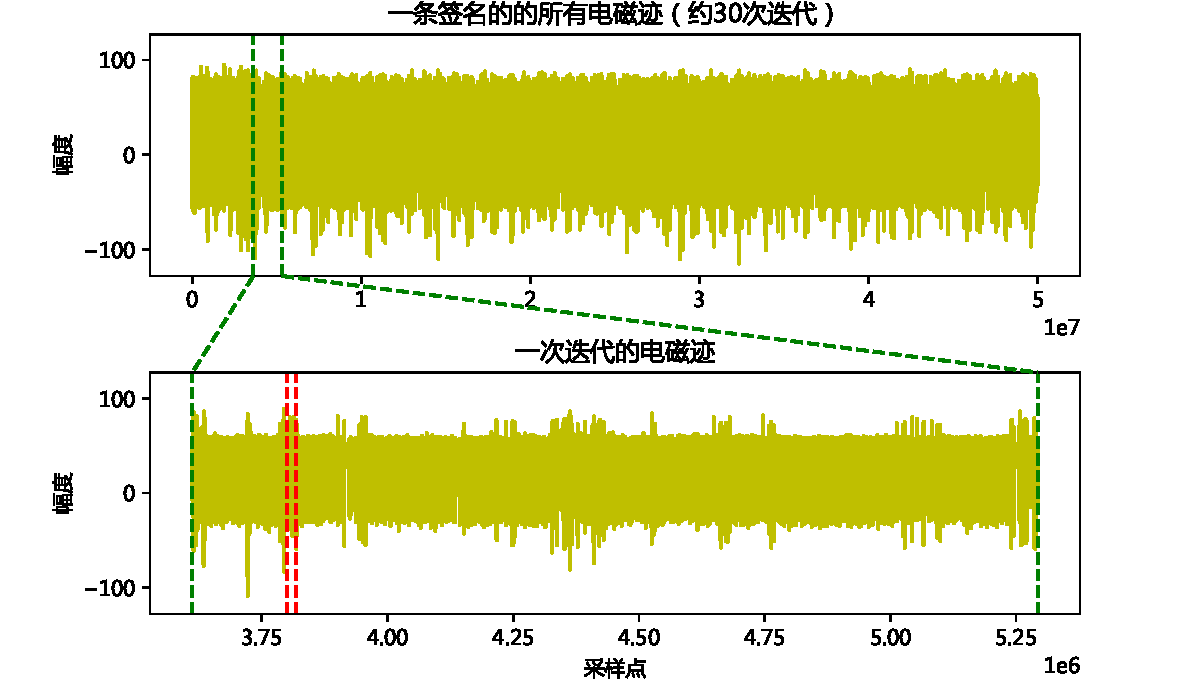
\includegraphics[width=\textwidth]{onetrs}
			\bicaption{\enspace ECDSA实现信息泄漏范围}{\enspace ECDSA Implementation EM Leakage Range}
			\label{fig:onetrs}
		\end{center}
	\end{figure}
	
	在阶段一,我们首先对电磁迹分块(对于本研究,第0至359个采样点的所对应的电磁迹的幅度构成第0个块,第360至719个采样点所对应的电磁迹的幅度构成第1个块,以此类推),每块的方差所构成的数列可以与电磁迹相对应,如\figureref{fig:halfphase1}的上、中两幅图所示。从图中可以看到,直观看来电磁迹中较粗的条带(如横坐标为400000附近的区域)所计算出的分块的方差也较大,较细的条带(如横坐标为392000附近的区域)所计算出的分块的方差也较小。这说明分块计算方差考虑到了电磁迹总体的变化趋势,这有助于进一步定位每次迭代的起止位置。
	
	在计算出每块的方差后,按照阈值执行量化和去抖动的操作,去抖动后的数列依然可以与电磁迹相对应,如\figureref{fig:halfphase1}的上、下两幅图所示。从图中可以看到,量化和去抖动后的数列所绘制的波形图依然体现了电磁迹总体变化的趋势,并且减小了后续分析的难度(从处理实数数列变为处理01数列)。但是此时的数列依然存在噪声,方波的数量对于每次迭代还是各不相同的,这使得如果仅以此作为辅助信息划分每一次迭代需要让程序频繁进行交叉验证,从而大幅增加时间消耗。
	
	\begin{figure}[!h]
		\begin{center}
			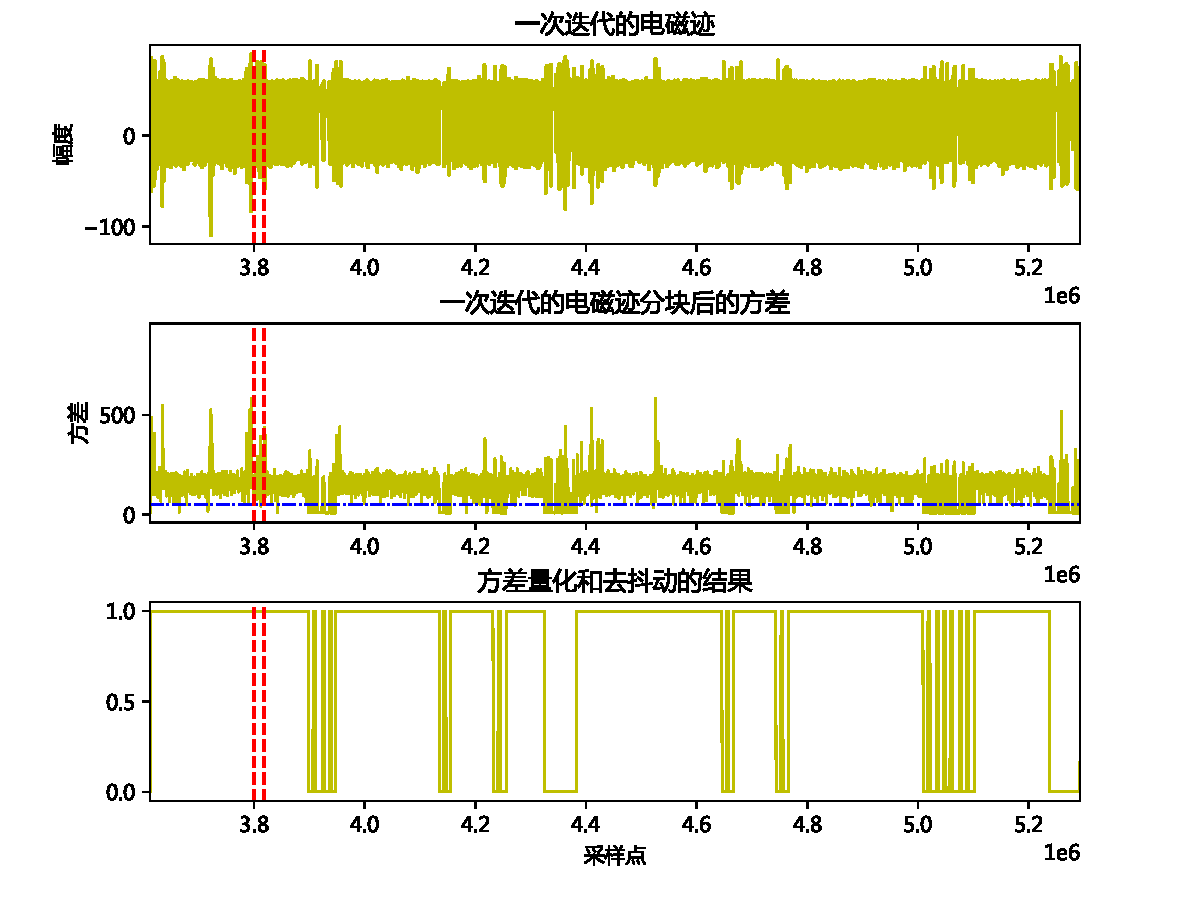
\includegraphics[width=\textwidth]{halfphase1}
			\bicaption{\enspace ECDSA实现电磁迹、电磁迹分块后的方差、方差量化和去抖动的结果}{\enspace ECDSA Implementation Raw Trace, the Variance of Trace Chunks and the Variance after Quantization and Anti-jitter}
			\label{fig:halfphase1}
		\end{center}
	\end{figure}

	为了消除方差量化和去抖动的结果中的噪声,我们需要对它做进一步处理。使用模糊函数减小结果中的噪声以及降低层次细节,最终模糊后的数列依然可以与电磁迹相对应,如\figureref{fig:fullphase1}的上、中两幅图所示。从图中可以看到,相比于模糊前,模糊后的数列所绘制的波形图变化更为平缓,偶然的噪声也因为平均了邻域的数值而被减弱。
	
	在进行模糊后,数列又从01数列变为实数数列,增加了分析的难度。按照新的阈值重新执行量化和去抖动的操作,最终的数列还是可以与电磁迹相对应,如\figureref{fig:fullphase1}的上、下两幅图所示。从图中可以看到,量化和去抖动仅消除了被模糊所减弱的噪声,减小了后续分析的难度而没有产生其他负面影响。

	随机选取部分计算结果,人工地对标注的信息泄漏范围和在阶段一之后计算出的辅助信息进行对比,发现他们的差值(如\figureref{fig:fullphase1}中下方的图,第一个下降沿横坐标与红色虚线横坐标的差值)几乎一致(标准差远小于均值)。因此我们认为阶段一之后可以准确划分出每次迭代,并找出其所对应的电磁迹的泄漏范围。
	
	\begin{figure}[!h]
		\begin{center}
			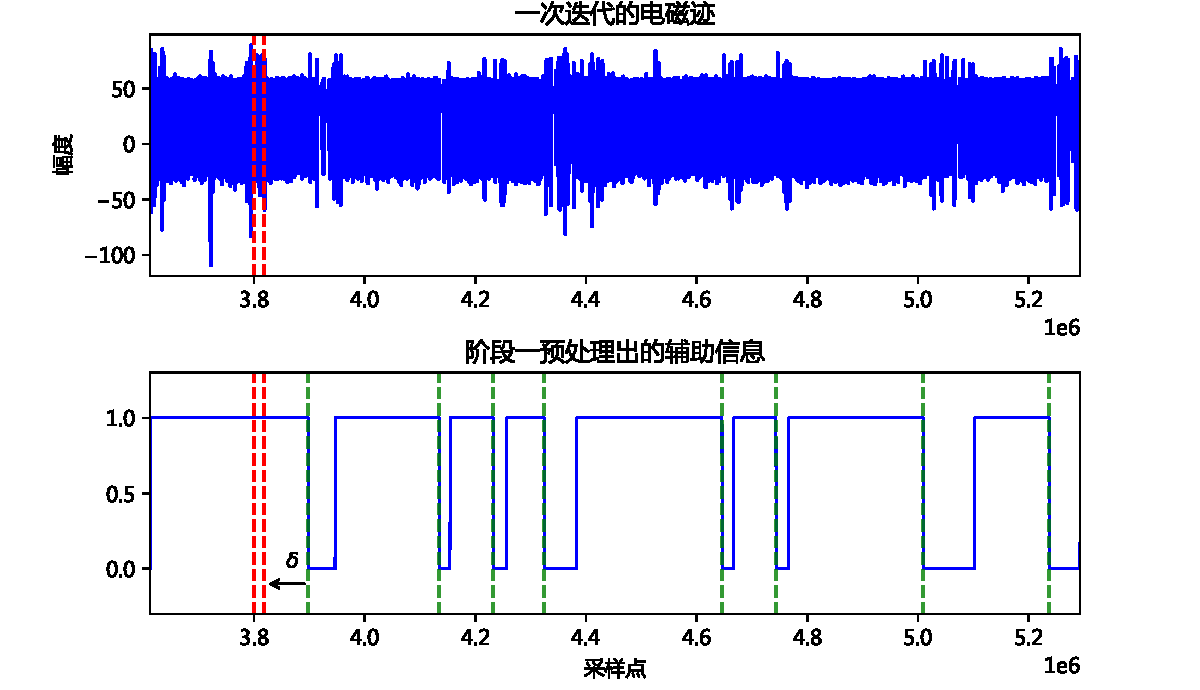
\includegraphics[width=\textwidth]{fullphase1}
			\bicaption{\enspace ECDSA实现电磁迹、方差量化去抖动并模糊的结果、方差量化去抖动并模糊后再量化去抖动的结果}{\enspace ECDSA Implementation Raw Trace, Variance after Quantization, Anti-jitter and Blurring and the Blurred Variance after Quantization and Anti-jitter again}
			\label{fig:fullphase1}
		\end{center}
	\end{figure}
	
	\begin{figure}[!h]
		\begin{center}
			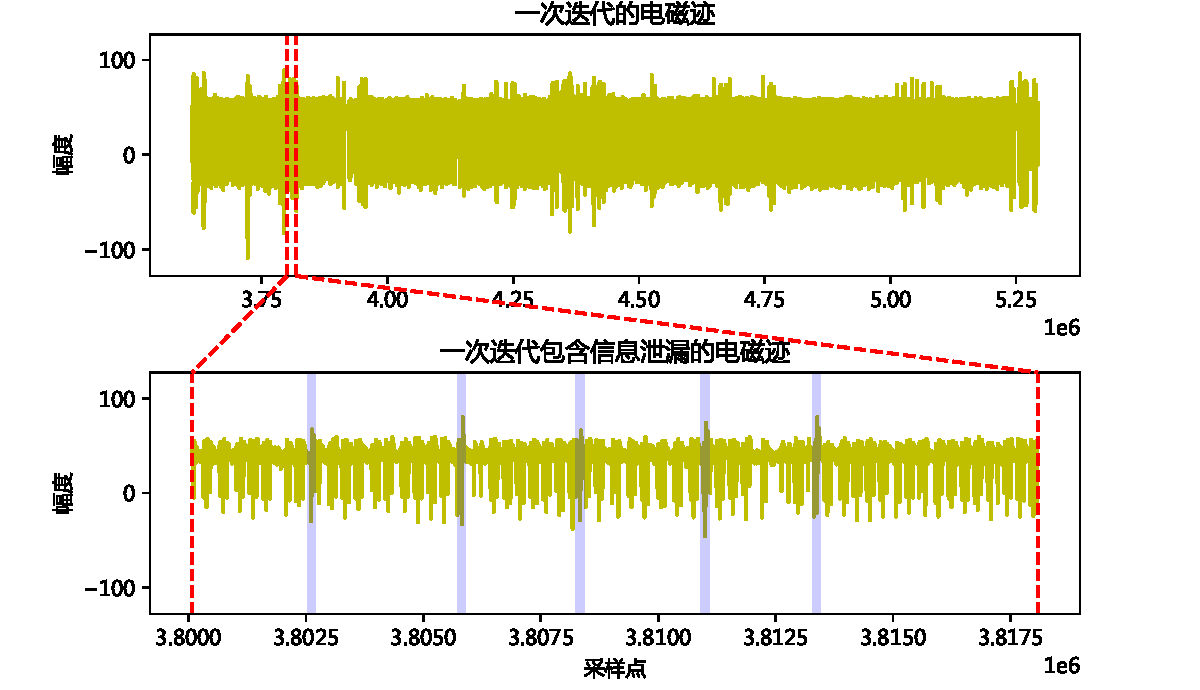
\includegraphics[width=\textwidth]{onetrsleak}
			\bicaption{\enspace ECDSA实现信息泄漏位置}{\enspace ECDSA Implementation EM Leak Positions}
			\label{fig:onetrsleak}
		\end{center}
	\end{figure}

	到目前为止,我们可以准确划分出每次迭代,并找出其所对应的电磁迹的泄漏范围,但是还是不能准确确定泄漏位置。\figureref{fig:onetrsleak}绘制了所采集到的一条电磁迹在人工标注的泄漏范围内的波形图,其中五处浅蓝色条带是人工标注的信息泄漏位置。我们期望在阶段二之后可以类似地找到信息泄漏位置。
	
	使用简单的统计信息难以找到信息泄漏位置。为了解决这个问题,我们使用更复杂的数学工具分析采样点之间内在的联系。我们构造了一个模版,计算模版与所有模版所确定的采样点的邻域各自的协方差作为统计指标用于后续分析。\figureref{fig:rhovscov}展示了使用同一个模版所计算出的协方差与相关系数。从图中可以看到人工标注的信息泄漏位置与相关系数曲线的峰值恰好对应,但是难以和相关系数曲线峰值对应。例如,人工标注的第四处信息泄漏,在协方差曲线的对应位置有显著的峰值,但是在相关系数曲线中对应位置没有特征使得此位置可以从其他假阳性中区分出来。
	
	\begin{figure}[!h]
		\begin{center}
			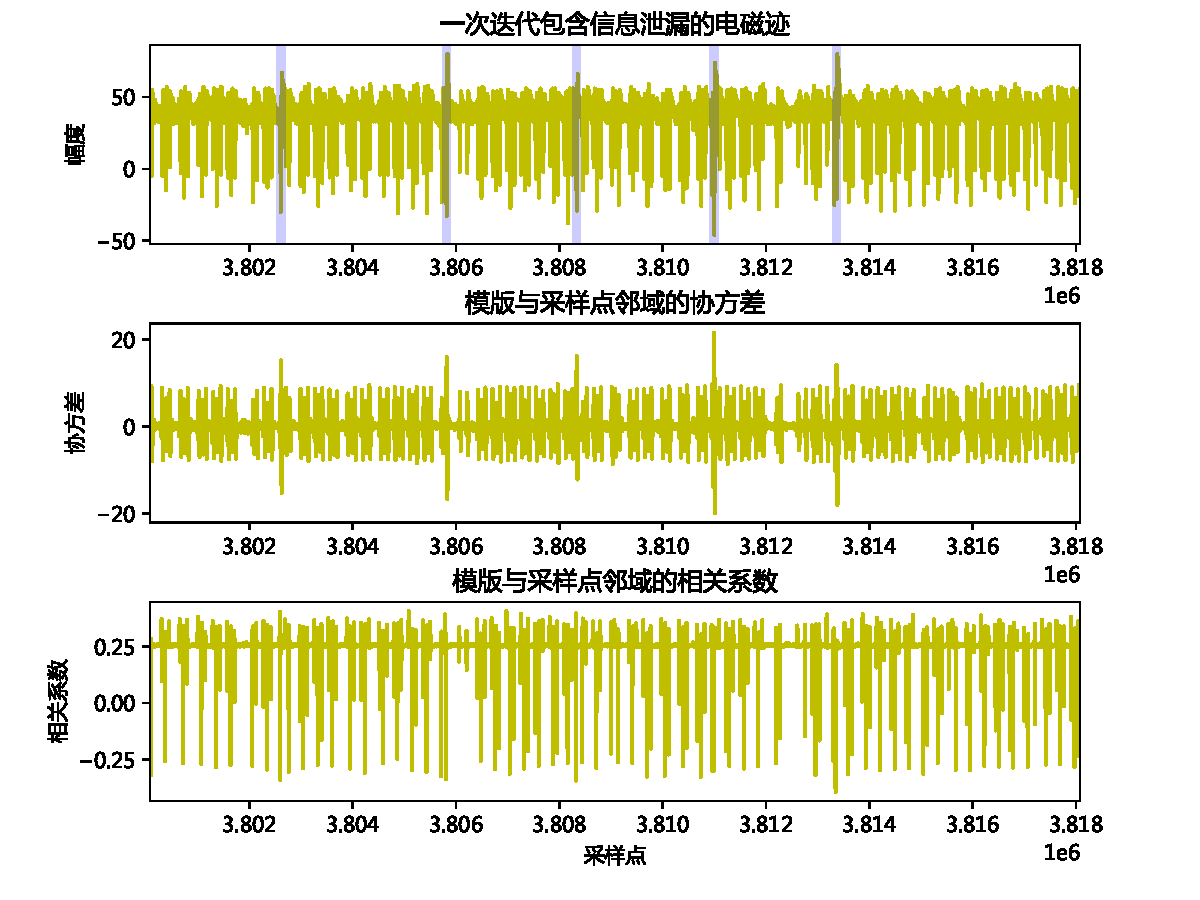
\includegraphics[width=\textwidth]{rhovscov}
			\bicaption{\enspace ECDSA实现信息泄漏及其对应的协方差与相关系数}{\enspace ECDSA Implementation EM Leakages and its Corresponding Covariance and Correlation Coefficient}
			\label{fig:rhovscov}
		\end{center}
	\end{figure}

	\begin{figure}[!h]
		\begin{center}
			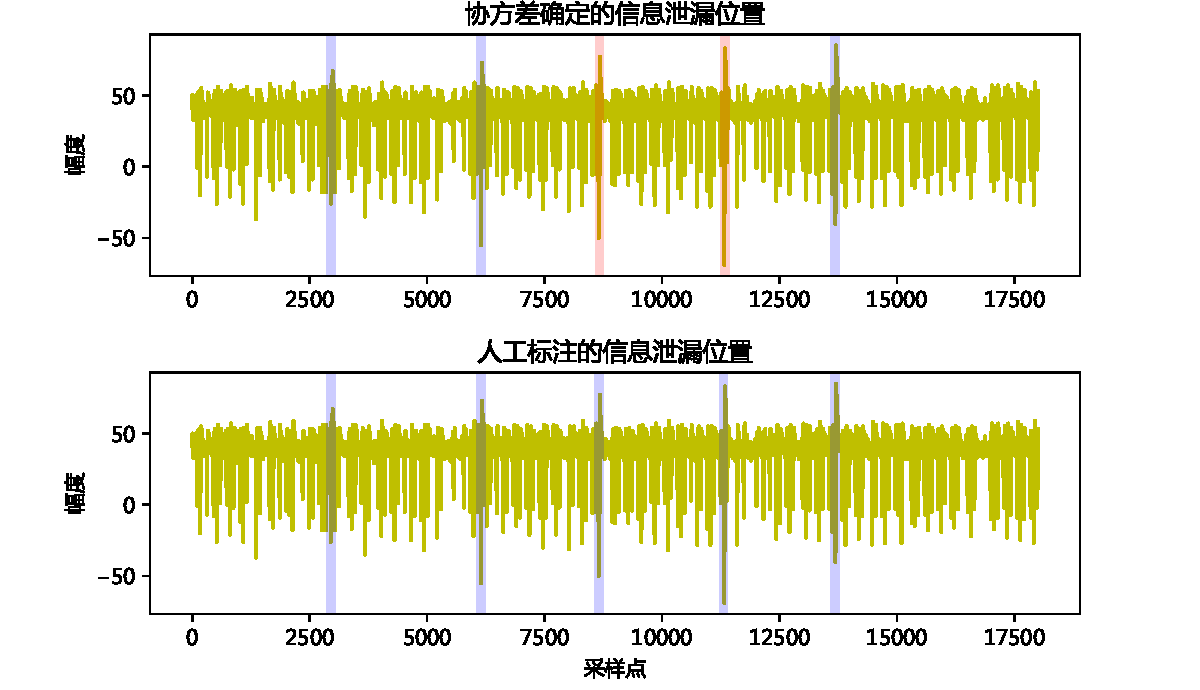
\includegraphics[width=\textwidth]{badmark}
			\bicaption{\enspace 计算出的错误信息泄漏位置和标注的信息泄漏位置的差异较小的情况}{\enspace Subtle Differences between Labeled and Wrongly Calculated Leak Positions}
			\label{fig:badmark}
		\end{center}
	\end{figure}
	
	尽管使用协方差已经帮助找到信息泄漏位置,但是我们在后续研究中发现以此确定的信息泄漏位置可能存在问题,如\figureref{fig:badmark}所示。从图中可以看到,协方差的前5个极值点所确定的信息泄漏位置中,红色条带标注位置是错误的,并不能对应到人工标注的泄漏位置。虽然图中看起来偏差不大,但对应的电磁迹片段和实际信息泄漏完全不符,这会导致后续恢复信息泄漏失败。出现偏差是因为取极值点操作不区分极大值点还是极小值点,从而引入一个系统误差。我们对这种系统误差进行人工统计,在取极值点之后判断是极大值点还是极小值点并据此进行校正,消除系统误差。
	
	除此之外,有一定信息泄漏存在变形的情况,这使得它对应的协方差并不是前5个极值,而是位于稍微靠后的位置,如第6大的极值(\figureref{fig:badmark2})。本研究尝试后发现,对于所采集的电磁迹,每次迭代取前9个极值点,有超过95\%的概率能找到五个极值点,这五个极值点校正后与人工标注的泄漏位置的几乎重合。
	
	\begin{figure}[!h]
		\begin{center}
			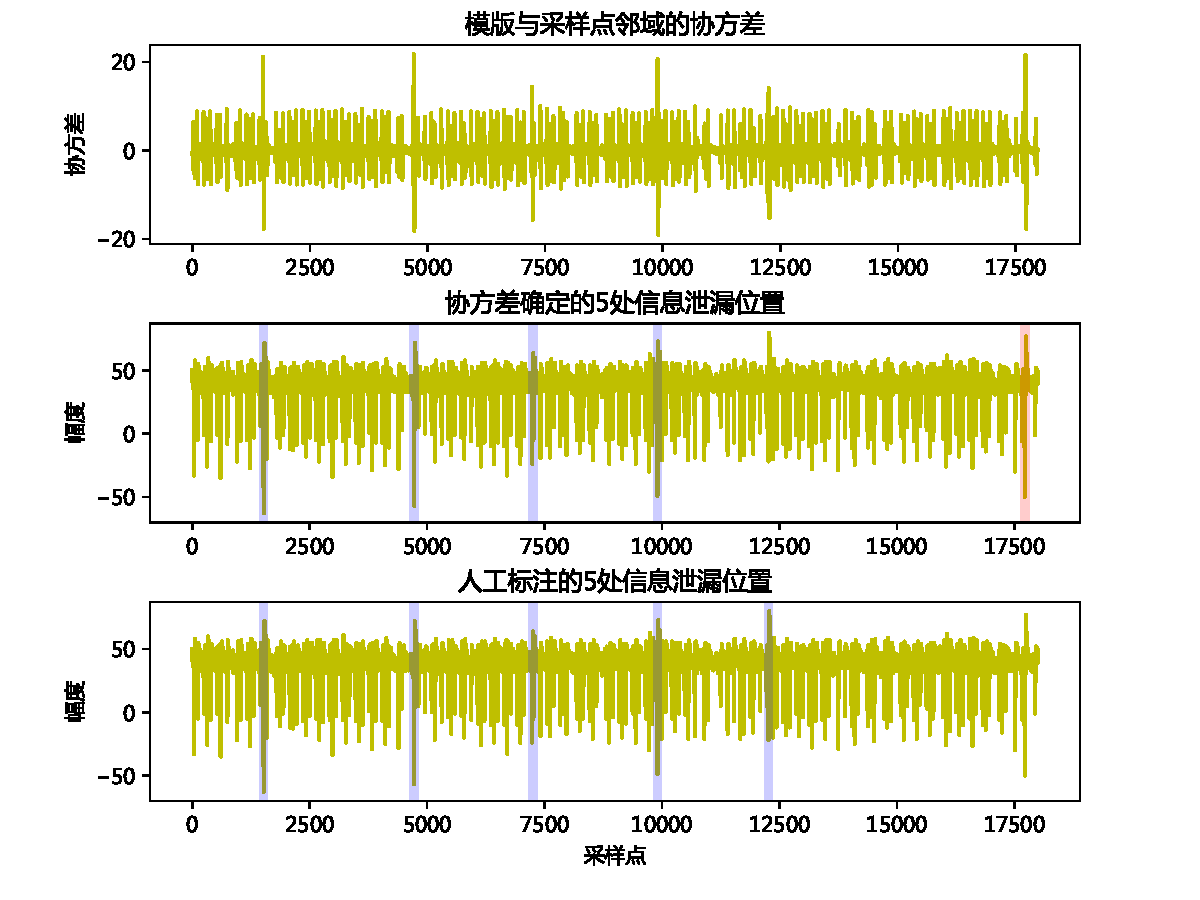
\includegraphics[width=\textwidth]{badmark2}
			\bicaption{\enspace 计算出的错误信息泄漏位置和标注的信息泄漏位置的差异较大的情况}{\enspace Substantial Differences between Labeled and Wrongly Calculated Leak Positions}
			\label{fig:badmark2}
		\end{center}
	\end{figure}

	为了准确刻画这种重合程度,本文对信息泄漏位置之间采样点的距离建立模版,如\figureref{fig:lambda10}所示。对于一次迭代所对应的多处泄漏,我们认为信息泄漏之间采样点的距离$\delta_0,\delta_1,\dots,\delta_9$应当服从正态分布。\figureref{fig:delta-l0-r1detail}展示了$\delta_0$前1000个样本的概率直方图,从完整的直方图中可以知道,对于大部分迭代所对应的电磁迹,使用协方差找到的第0处信息泄漏位置和第1处信息泄漏位置相隔的采样点个数在3199左右,但是还存在极少数的情况会找错第0处泄漏位置或第1处泄漏位置,这对应于直方图在某些异常的位置(如2516)频数不为0。将数据比较集中的部分进行放大,我们进一步发现直方图可以大致分为三个区间:[3170,3191),[3191,3209)和[3209,3230)。对于区间[3191,3209),它是样本最集中的区域,频数直方图和竖直拉伸后的正态分布曲线(图中蓝色曲线)比较重合,这说明假设$\delta_0$服从正态分布是合理的。另外两个区间不是样本最集中的区域,但是频数直方图也和竖直拉伸后的正态分布曲线(图中黄色、程色曲线)比较重合。实际上,三个区间分别对应这样的情况:
	
	\begin{itemize}
		\item 如果第0处信息泄漏位置是通过协方差取极小值点得出,而第1处信息泄漏位置是通过协方差取极大值点得出,那么这向第0、1处信息泄漏之间采样点的距离中引入了一个小于0的系统误差,$\delta_0$的样本值很可能落在[3170,3191);
		\item 如果第0、1处信息泄漏位置通过协方差都取极大值点或都取极小值点得出,这没有向第0、1处信息泄漏之间采样点的距离引入系统误差,那么$\delta_0$的样本值很可能落在[3191,3209);
		\item 如果第0处信息泄漏位置是通过协方差取极大值点得出,而第1处信息泄漏位置是通过协方差取极小值点得出,那么这向第0、1处信息泄漏之间采样点的距离中引入了一个大于0的系统误差,$\delta_0$样本值很可能落在[3209,3230)。
	\end{itemize}

	这进一步说明取极值点操作应当区分极大值点还是极小值点并及时校正,从而避免系统误差。校正之后,频数直方图数据分布变得更集中了。对于$\delta_1,\delta_2,\dots,\delta_9$,他们的情况和$\delta_0$类似,唯一不同之处在于正态分布的均值和方差一般是不同的,如\appfigureref{appfig:deltaall}所示,因此总共需要计算10次时间的模版。
	
	%视为我们人工对少量(10条电磁迹合计约300次迭代)电磁迹的信息泄漏位置进行标注,统计这些位置之间的差值的均值和方差,作为刻画重合程度的模版。
	
	\begin{figure}[!h]
		\begin{center}
			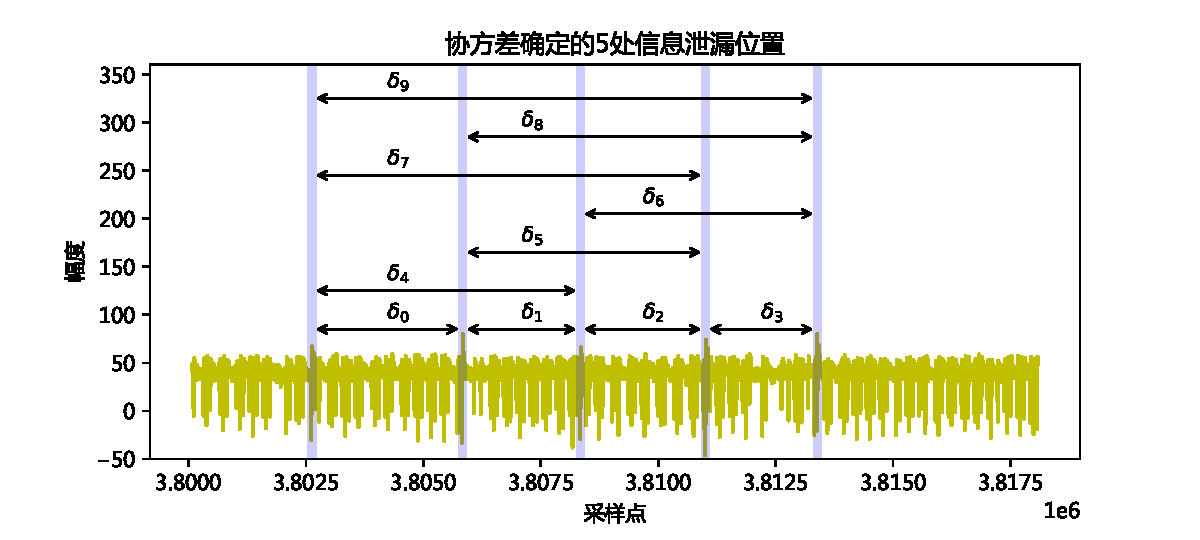
\includegraphics[width=\textwidth]{lambda10}
			\bicaption{\enspace 信息泄漏位置之间的距离示意图}{\enspace Demostration of Calculating Distance between Leak Positions}
			\label{fig:lambda10}
		\end{center}
	\end{figure}
	
	\begin{figure}[!h]
		\begin{center}
			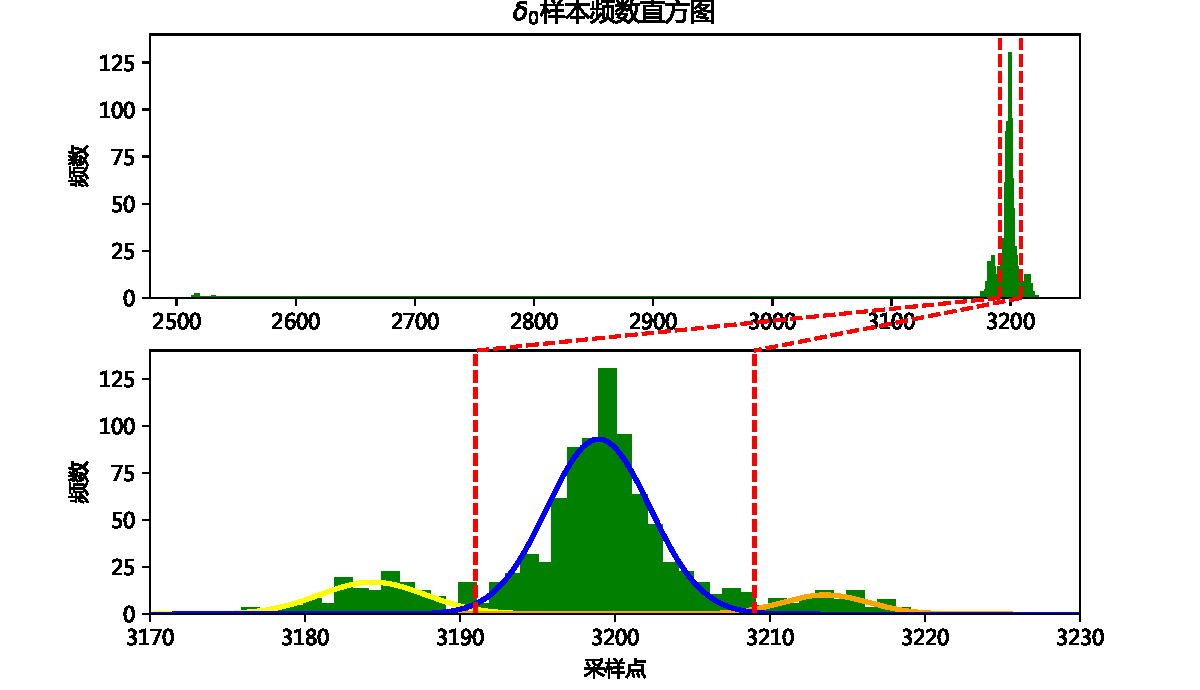
\includegraphics[width=\textwidth]{delta-l0-r1detail}
			\bicaption{\enspace 1000个$\delta_0$的样本频数直方图}{\enspace Frequency Histogram of 1000 $\delta_0$ Samples}
			\label{fig:delta-l0-r1detail}
		\end{center}
	\end{figure}

	使用校正后的前9个极值点以及预计算的模版,\algorithmref{alg:checkdelta}可以筛选出符合模版的极值点,进而确定信息泄漏位置,如\figureref{fig:select9}所示。虽然前9个极值点中一定会有错误的,但是进行模版检查之后可以排除这种错误,从而准确选出理论上会对应信息泄漏的5个极值点。在极少的情况下(占所有情况的比例少于5\%),找不到符合模版的极值点,因此无法确定某一次迭代的信息泄漏位置,也就无法恢复此次迭代的信息泄漏。需要注意的是,这种情况不会直接导致攻击失败,只是会增加找到可利用(连续4比特)的敏感信息泄漏的难度。
	
	\begin{figure}[!h]
		\begin{center}
			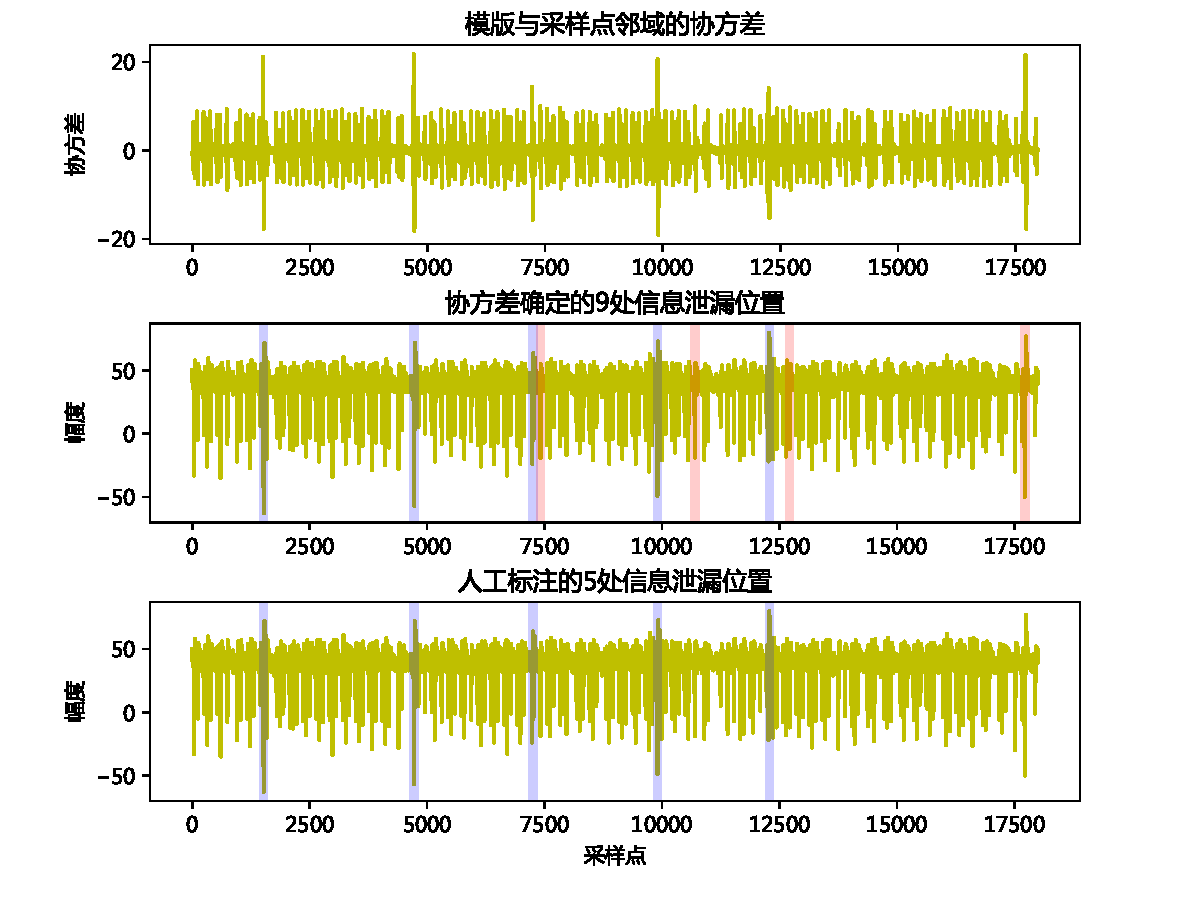
\includegraphics[width=\textwidth]{select9}
			\bicaption{\enspace 协方差极值点不能确定的信息泄漏位置的情况}{\enspace Failing to Determine the Leak Position using Argmax of Covariance}
			\label{fig:select9}
		\end{center}
	\end{figure}

	随机选取部分计算结果,人工地对标注的信息泄漏位置和在阶段二之后计算出的信息泄漏位置进行对比,根据结果认为阶段二达到了预期效果,可以准确确定信息泄漏位置。获得了信息泄漏位置后,我们从相应位置及其邻域\footnote{邻域的大小可以自行设定。在本研究中,邻域设定为以当前位置为中心,左右各150个采样点的区间。}提取电磁迹并重新对采样点编号。\figureref{fig:aligndemo}绘制了提取出的每次迭代的第二处包含信息泄漏的电磁迹,上图是500条中间值$\leakedmultiplier_i=1$的电磁迹以及500条中间值$\leakedmultiplier_i=3$的电磁迹,下图是这1000条能量迹进行TVLA的结果。从下图TVLA结果在第140个采样点取得极值且超过阈值4.5,因此我们有超过99.999\%的把握认为提取出的电磁迹在第140个采样点处存在信息泄漏。上图中曲线的颜色的深浅可以体现某一类能量迹的集中程度,可以看出,$\leakedmultiplier_i=1$所对应的电磁迹在第140个采样点的幅度总体来说是比$\leakedmultiplier_i=3$所对应的幅度大,这与TVLA的结果是一致的。
	
	\begin{figure}[!h]
		\begin{center}
			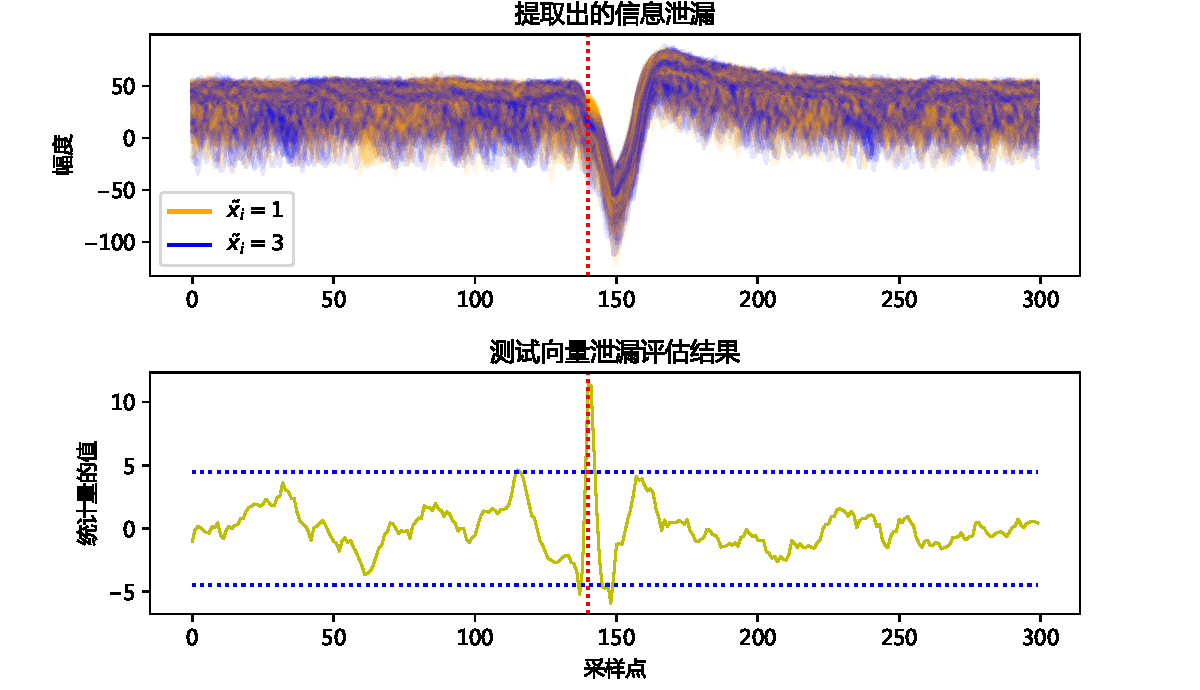
\includegraphics[width=\textwidth]{aligndemo}
			\bicaption{\enspace 每次迭代包含第二处信息泄漏的电磁迹及其TVLA结果}{\enspace Subtraces Containing the Second Leakage of Each  Iterations and their TVLA Result}
			\label{fig:aligndemo}
		\end{center}
	\end{figure}

	在评估阶段,我们只能知道每个$\tilde \nonce_i$的值但是不能准确知道每个$\leakedmultiplier_i$的值,如\tableref{tab:partialknownti}所示。我们从所有迭代含有信息泄漏的电磁迹中过滤出了对应的$\leakedmultiplier_i$完全确定的电磁迹(即从所有电磁迹中只选出对应的$\tilde \nonce_i\neq0$的电磁迹)并使用TVLA进行泄漏检测。对于每次迭代包含其它信息泄漏的电磁迹,不同中间值$\leakedmultiplier_i$之间TVLA结果见\appfigureref{appfig:aligndemoall}。
	
	\begin{table}[!htb]
		\bicaption{\enspace 评估时可以推断的$\leakedmultiplier_i$的信息}{\enspace Deduced $\leakedmultiplier_i$ for Evaluation}
		\label{tab:partialknownti}
		\centering
		\begin{subtable}{\twof\textwidth}
			\centering
			\begin{tabular}{cc|ccc}
				\hline
				\multicolumn{2}{c|}{\multirow{2}{*}{$\Pr[\leakedmultiplier_i=v|\tilde \nonce_i=w]$}} & \multicolumn{3}{c}{$v$} \\
				%\cline{3-5}
				\multicolumn{2}{c|}{}& 1 & 2 & 3 \\
				\hline
				\multirow{4}{*}{$w$} & 0 & $\frac12$ & $\frac14$ & $\frac14$ \\
				%\cline{2-5}
				& 1 & 1 & 0 & 0 \\
				%\cline{2-5}
				& 2 & 0 & 1 & 0 \\
				%\cline{2-5}
				& 3 & 0 & 0 & 1 \\
				\hline
			\end{tabular}
			\subcaption{$\leakedmultiplier_i$的条件分布列}
			\label{tab:partialknowntidetail}
		\end{subtable}\hfill
		\begin{subtable}{\twof\textwidth}
			\centering
			\begin{tabular}{c|cc}
				\hline
				$\tilde \nonce_i$数值&能否知道$\leakedmultiplier_i$数值&$\leakedmultiplier_i$数值\\
				\hline
				0 & 否 & /\\
				1 & 是 & 1\\
				2 & 是 & 2\\
				3 & 是 & 3\\
				\hline
			\end{tabular}
			\subcaption{由$\tilde \nonce_i$可以推断的$\leakedmultiplier_i$的信息}
			\label{tab:partialknownticonclusion}
		\end{subtable}
	\end{table}

	总的来说,进行阶段二之后我们可以成功提取包含信息泄漏的电磁迹且能通过TVLA检测出存在信息泄漏。经过阶段一和阶段二,提取出包含信息泄漏的电磁迹后,还需要从中恢复信息泄漏才能完成对智能卡ECDSA实现的侧信道分析整个流程。
	\section{自适应数据增强方法在ECDSA算法实现分析中的应用}
	\subsection{实验设置}
	\subsubsection{主控制器设置}
	\subsubsection{数据增强单元设置}
	\subsubsection{攻击评估单元设置}
	\subsubsection{基于深度学习的侧信道攻击模型设置}
	\subsection{自适应数据增强方法在ECDSA算法实现分析中的实证研究}
	\subsubsection{自适应数据增强方法的技术效果}
	\subsubsection{无数据增强的技术效果}
	\subsection{讨论与分析}
	总表对比结果。
}